\documentclass[ngerman,aspectratio=1610,12pt]{beamer}
\usepackage[utf8]{luainputenc}
\usepackage[TS1,T1]{fontenc}
\usepackage{babel}
\usepackage{listings}
\usepackage{graphicx}
\usetheme[pagenum,noddc,cd2018]{tud}

\usepackage{xcolor}
\usepackage{listings}

\title[Fuzzing]{Fuzzing\protect\\\mdseries Ein kurzer Überblick\strut}
\author{~}
\einrichtung{Technische Universität Dresden}
\fachrichtung{Fakultät Informatik}
\professur{Professur für Betriebssysteme}
\datecity{Dresden}
\date{11. Januar 2019}

\AtBeginSection[]{\partpage{\usebeamertemplate***{part page}}}
\begin{document}
\maketitle
\setbeamertemplate{page number in footline}[page][text and total]
\frame{\frametitle{Inhalt}\tableofcontents}


\section{Grundidee}
\begin{frame}{Grundidee}
  \begin{block}{Grundidee}
      \begin{enumerate}
    \item Füttern von Programm mit zufällige Daten
    \item Protokollieren von  Programmabstürzen und deren Ursachen 
  \end{enumerate}
  \end{block}
 
  \begin{block}{Erste wissenschaftliche Veröffentlichung}
    Barton Miller et. al. (1989): "`An Empirical Study of the Reliability of UNIX Utilities"'
  \end{block}
\end{frame}


\section{Vor- und Nachteile}
\begin{frame}{Vor- und Nachteile}
  \begin{itemize}
    \item Vorteile:
    \begin{itemize}
      \item Implementierung einfach
      \item Fehlerdetektion auch in Randfällen sowie außerhalb der Spezifikation
      \item Wartungsaufwand zum Finden von Abstürzen gering
    \end{itemize}
    \item Nachteile:
    \begin{itemize}
      \item Keine Garantie für vollständige Fehleridentifizierung
      \item Robustheitsprüfung, aber keine Verifikation der Ergebnisse
      \item Notwendigkeit einer manuelle Absturzanalyse
      \item Rechenaufwand hoch
    \end{itemize}
  \end{itemize}
\end{frame}

\section{Techniken}
\begin{frame}{Techniken}{Übersicht\\}
  \begin{itemize}
    \item Was wird gefuzzt?
    \begin{itemize}
      \item Programme mittels Dateien, \texttt{stdin}, Netzwerk, ...
      \item Betriebssysteme mittels Syscalls
      \item Hardware
    \end{itemize}
  
    \item Wie werden die Daten generiert?
    \begin{itemize}
      \item Zufälliges Fuzzing
      \item Mutationsbasiertes Fuzzing
      \item Regelbasiertes Fuzzing
      \item Instrumentiertes Fuzzing
    \end{itemize}
  \end{itemize}    
\end{frame}

\subsection*{Zufälliges Fuzzing}
\begin{frame}{Techniken I}{Zufälliges Fuzzing \\{\large (random fuzzing)}}
  \begin{itemize}
    \item Generierung zufälliger Daten und Verarbeitung durch Programm \\\texttt{cat \textbackslash dev\textbackslash urandom |  programm\_to\_fuzz}
    \item Vorteil: 
    \begin{itemize}
      \item Sehr einfach
    \end{itemize}
    \item Nachteile: 
    \begin{itemize}
      \item Nur Entdeckung einfacher Fehler
    \end{itemize}
  \end{itemize}
\end{frame}

\subsection*{Mutationsbasiertes Fuzzing}
\begin{frame}{Techniken II}{Mutationsbasiertes Fuzzing \\{\large(mutation based fuzzing)}}
  \begin{itemize}
    \item Erstellung einer Sammlung von Testdaten (Testkorpus)
    \item Mutation der Daten im Testkorpus
    \item Vorteil:
    \begin{itemize}
      \item Implementierung simpel
      \item Findet viele Fehler
    \end{itemize} 
    \item Nachteile:
    \begin{itemize}
      \item Große Abhängigkeit von Testdatenauswahl
    \end{itemize}
    \item Tools: \texttt{zzuf}, \texttt{Radamsa}
  \end{itemize}
\end{frame}

\subsection*{Regelbasiertes Fuzzing}
\begin{frame}{Techniken III}{Regelbasiertes Fuzzing \\{\large (generation based fuzzing)}}
  \begin{itemize}
    \item Erstellung einer Datenbeschreibung aus Spezifikation %(Modell, Grammatik)
    \item Generierung zufälliger Sequenzen aus Beschreibung
    \item Vorteil:
    \begin{itemize}
      \item Entdeckung komplexer Logik- und Protokollfehler
    \end{itemize}
    \item Nachteile:
    \begin{itemize}
      \item Hoher Aufwand der Beschreibungserstellung
      \item Existenz einer Spezifikation nötig
      \item Starke Abhängigkeit von Beschreibungsqualität
    \end{itemize} 
    \item Tools: \texttt{Peach Fuzzer}, \texttt{Dharma}
  \end{itemize}
\end{frame}

\subsection*{Instrumentiertes Fuzzing}
\begin{frame}{Techniken IV}{Instrumentiertes Fuzzing \\{\large (coverage guided fuzzing)}}
  \begin{itemize}
    \item Beobachtung der Codeausführung
    \item Mutation der Daten anhand des Feedbacks
    \item Vorteile:
    \begin{itemize}
      \item Hohe Effizienz
      \item Hohe Code-Abdeckung
      \item Ermöglicht Testkorpus- sowie Testfallminimierung
    \end{itemize}
    Nachteil:
    \begin{itemize}
      \item Leichte Verschlechterung der Performance
    \end{itemize}
    \item Tools: \texttt{AFL}, \texttt{libFuzzer}, \texttt{honggfuzz}
  \end{itemize}
\end{frame}


\subsection*{Datenmutation}
\begin{frame}{Techniken V}{Datenmutation\\}
  \begin{itemize}

    \item Vollständiges Durchsuchen nicht möglich: \\ $2^{32}$ Möglichkeiten $\rightarrow$ 50 Tage fuzzen
    \item Einschränkung des Suchraums durch:
    \begin{itemize} 
      \item Bit-Flips und -Shifts
      \item Zahlenersetzung (0, 1, -1, \texttt{MAXINT - 1}, \texttt{MAXINT}, \texttt{NaN}, \texttt{Inf})
      \item Addition oder Subtraktion bestehender Zahlen
      \item Einfügen interessante Zeichenketten:
      \begin{itemize}
        \item Sehr lange oder komplett leere Zeichenketten (\texttt{''}, \texttt{128*'a'})
        \item Spezielle Zeichen (\texttt{\textbackslash 0}, \texttt{\textbackslash n})
        \item Pfade (\texttt{../../../../../../../etc/shadow})
        \item Format Strings (\texttt{\%s\%s\%s\%s}, \texttt{\%x \%x \%x}) % format string attacks
      \end{itemize}
    \end{itemize}
  \end{itemize}
\end{frame}


\begin{frame}{Techniken V}{Datenmutation\\}
  \begin{center}
    \begin{columns}[T]
      \begin{column}{.5\textwidth}
        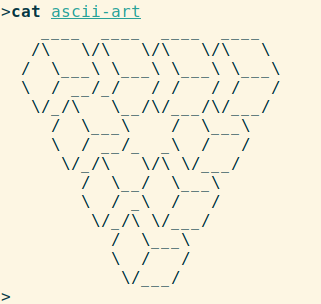
\includegraphics[height=0.55\textheight]{images/zzuf1}      
      \end{column}
      \begin{column}{.5\textwidth}
        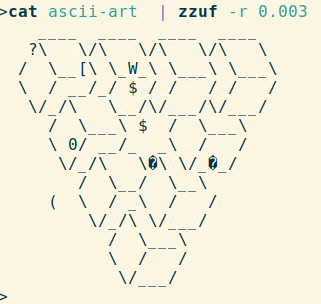
\includegraphics[height=0.55\textheight]{images/zzuf2}      
      \end{column}   
    \end{columns}
    \vspace{0.5em}
    \hspace{-5em}Zufällige Bitflips mit \texttt{zzuf}
  \end{center}
  
  
\end{frame}
\begin{frame}{Techniken V}{Datenmutation\\}
  \begin{center}
    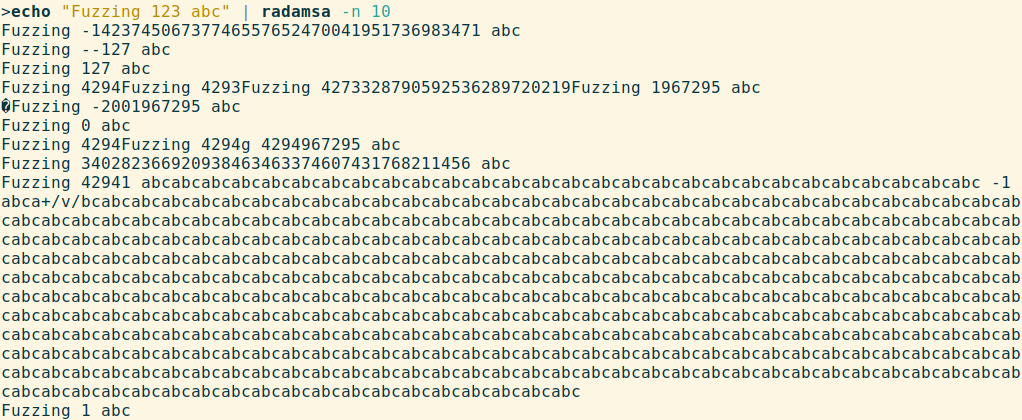
\includegraphics[width=0.8\textwidth]{images/radamsa}
    Datenmanipulation mittels \texttt{radamsa} 
  \end{center}
  
\end{frame}


\subsection*{Sanitizer}
\begin{frame}{Techniken VI}{Sanitizer\\}
  \begin{itemize}
    \item Problem: Kein sofortiger Programmabsturz durch bestimmte Fehler
    \item Lösung: Verwendung eines Sanitizers
    \begin{itemize}
      \item Ergänzung des Codes um zusätzliche Überprüfung von Argumenten
    \end{itemize} 
    \item Nachteil: Erhöhung des Rechen- und Speicherbedarfs
    \item Entwickelte Sanitizer:
    \begin{itemize}
      \item AddressSanitizer (ASan) % (Out-of-bounds memory access, Double free, Use-after-free)
      \item UndefinedBehaviorSanitizer (UBSan)% (divide by zero, integer overflow)
      \item MemorySanitizer % (uninitilisierte Lesevorgänge)
      \item LeakSanitizer % (Memory leaks)
      \item ThreadSanitizer % (Data races)
    \end{itemize}
  \end{itemize}
\end{frame}

\begin{frame}{Techniken VI}{Sanitizer\\ }
  \begin{center}
    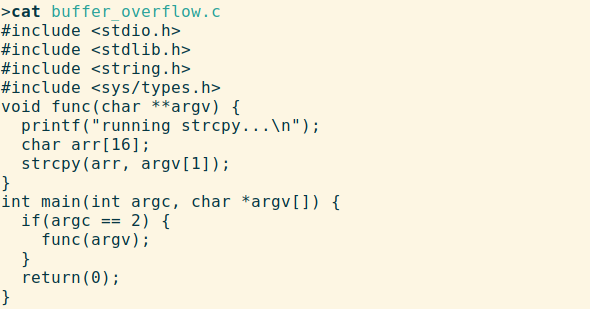
\includegraphics[width=0.7\textwidth]{images/buffer_overflow1}
    Demonstrationsprogramm
  \end{center}
\end{frame}

\begin{frame}{Techniken VI}{Sanitizer\\}
  \begin{center}
    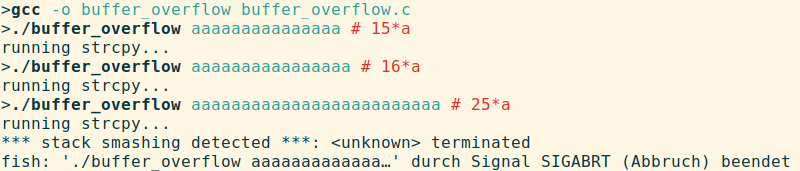
\includegraphics[width=0.8\textwidth]{images/buffer_overflow2}\\
    \vspace{1.5em}
    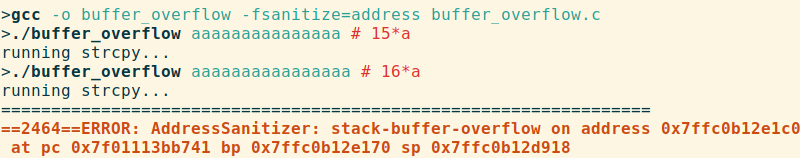
\includegraphics[width=0.8\textwidth]{images/buffer_overflow3}
    Kompilierung und Ausführung mit und ohne Sanitizer
  \end{center}
\end{frame}




% TODO hinzufügen:
% * skalieren wichtig -> soll auf 100 Cores laufen können (Intel Edison 1W/Board, VMs, VPS)
% * richtige Angriffsfläche und Attackart wählen
\subsection*{Tipps}
\begin{frame}{Techniken VII}{Tipps\\}
  \begin{itemize}

    \item Abwägung Fuzzing-Geschwindigkeit gegenüber Fuzzing-Effizienz \\ Anzahl gefunder Fehler = Programmausführungen * Sucheffizienz
    \item Verwendung von Sanitizern % Gentoo mit ASan kompiliert --> bei normaler Benutzung haben fast alle Programme Bugs
    \item Teilweise Codeanpassungen nötig \\ (Deaktivierung von Checksummen) 
  \end{itemize}
\end{frame}


\section[Tools]{Tools:\protect\\\mdseries American fuzzy lob, libFuzzer, ...\strut}
\begin{frame}{Tools: AFL und libFuzzer}
  \begin{itemize}
    \item American fuzzy lop-Entwicklung durch Michal Zalewski 
    \item libFuzzer-Entwicklung durch LLVM-Community
    \item Instrumentieren Code, erreichen hohe Code-Abdeckung
    \item Entdeckung sehr vieler Fehler in fast allen Programmen
    \item Entdeckung von Heartbleed einfach möglich
  \end{itemize}
\end{frame}


\begin{frame}{Tools}{AFL und libFuzzer}
  \begin{columns}[T] 
    \begin{column}{.5\textwidth}
      \texttt{AFL}
      \begin{itemize}
        \item Sehr schnelles Aufsetzen \\ (\textasciitilde 5 Minuten)
        \item Übergabe der Daten per \texttt{stdin} oder Datei
        \item Gray- und White-Box-Fuzzing
        \item Standard: Start vieler Prozesse
        \item Möglichkeit des In-Prozess-Fuzzings
      \end{itemize}
    \end{column}
    \hfill%
    \begin{column}{.5\textwidth}
      \texttt{libFuzzer}
      \begin{itemize}
        \item Schnelles Aufsetzen \\ (\textasciitilde $\frac{1}{2}$ Stunde)
        \item Übergabe der Daten durch Helferprogramm
        \item White-Box-Fuzzing
        \item Kompilierung mit \texttt{clang} notwendig
        \item schnell durch In-Prozess-Fuzzing 
      \end{itemize}
    \end{column}
  \end{columns}
\end{frame}

\subsection*{Quickstart}
\begin{frame}{Tools}{AFL und libFuzzer}
  \textbf{Quickstart  AFL:}
  \begin{itemize}
    \item Kompilierung:  \texttt{CC=afl-gcc ./configure --disable-shared}
    \item Ausführung: \texttt{afl-fuzz [...] ./programm\_to\_fuzz}
  \end{itemize}

  \textbf{Quickstart libFuzzer:}
  \begin{itemize}
    \item Implementierung des Helferprogramms: 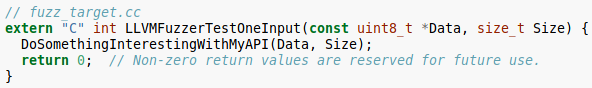
\includegraphics[width=0.9\textwidth]{images/libfuzz-quickstart}
    \item Kompilierung: \texttt{clang -fsanitize=fuzzer fuzz\_target.c}
    \item Ausführung: \texttt{./a.out [...]}
  \end{itemize}
\end{frame}




\subsection*{Kernel Fuzzing}
\begin{frame}{Tools}{Kernel-Fuzzer}
  \begin{itemize}
    \item \texttt{syzkaller}
    \begin{itemize}
      \item Entwicklung durch Google
      \item Instrumentiertes Fuzzing
      \item Start des Systems in VM und Fuzzing der Syscalls
    \end{itemize}
    \item Alternative: \texttt{trinity} 
  \end{itemize}
\end{frame}

\subsection*{Weitere Tools}
\begin{frame}{Tools}{Weitere Tools}
  \texttt{Sandsifter}
  \begin{itemize}
    \item Fuzzing von CPU-Instruktionen
    \item Entdeckung von Bugs in Disassemblern, Emulatoren, Hypervisorn sowie x86-Chips 
  \end{itemize}
  
  
  \texttt{ClusterFuzz} und OSS-Fuzz-Projekt
  \begin{itemize}
    \item Google-Entwicklung zum Fuzzing von Chrome
    \item Verteiltes Fuzzing auf hunderten Kernen
    \item OSS-Fuzz: Fuzzing verbreiteter  Open-Source-Software
  \end{itemize}
\end{frame}

\begin{frame}{}
  \centering \Huge
  \textbf{Fragen?}
\end{frame}
\end{document}
